% Chapter 11 -- Symbolic Programming

\chapter{Symbolic Programming}
\TallC{All} symbolic programming is based on \textbf{rules} --- a set of generalized instructions that tells the computer how to transform one set of \textbf{tokens} into another. An assembler, \textit{e.g.}, inputs a series of machine instructions in mnemonic form and outputs a series of numbers that represent the actual machine instructions in executable form. A FORTH compiler translates a definition into a series of addresses of previously defined objects. Even higher on the scale of complexity, a FORTRAN compiler inputs high-level language constructs formed according to a certain \textbf{grammar} and outputs an executable program in another language such as assembler, machine code or C.

What do rules have to do with scientific problem-solving? The crucial element in the rule-based style of programming is the ability to specify general \textbf{patterns} or even classes of patterns so the computer can recognize them in the input and take appropriate action.

For example, in a modern high-energy physics experiment the rate at which events (data) impinge on detectors might be $10^{7}$ discrete events per second. Since each event might be represented by 5-10 numbers, the storage requirements for recording the results of a search for some rare process, lasting 3-6 months of running time, might be $10^16$ bytes, or $10^7$ high-capacity disk drives! Clearly, so much storage is out of the question and most of the incoming data must be discarded. That is, such experiments demand extremely fast filtering methods that can determine - in 10-20$\mu$sec - whether a given event is interesting. The criteria for "interesting" may be quite general and may need to be changed during the running of the experiment. In a word, they must be specified by some form of pattern recognition program rather than hard-wired.

Another area where pattern recognition helps the scientist is computer algebra. Closely related is the ability to translate mathematical formulae into machine code. So far we have stressed a FORTH programming style natural to that language, namely postfix notation, augmenting it primarily for readability or abstracting power. It cannot be denied, however, that sometimes it is useful simply to be able to write down a mathematical formula and have it translated automatically into executable form. This chapter develops the tools for symbolic programming and illustrates their use with a typical algebra program and a simple FORmula TRANslator.

\subsection{Rules}
Before we can specify rules we need a language to express them in. We need to be able to describe the \textbf{grammar} of the rules in some way. The standard notation states rules as \textbf{regular expressions\sepfootnote{11_01}}. The following rules describing some parts of FORTRAN illustrate how this works.

\begin{verbatim}
\ Rules for FORTRAN

\ NOTATION:
\ |         -> "or"
\ ^         -> "unlimited repetitions"
\ ^n        -> "0-n repetitions"
\ Q         -> "empty set"
\ &         -> + | -
\ %         -> * | /
\ <d>       -> "digit"

\ NUMBERS:
\ <int>     -> {-|Q} {<d> <d> ^8}
\ <exp't>   -> {dDeE} {&|Q}{<d> <d> ^2} | Q
\ <fp\#>    -> {-|Q}{ <d> | Q} . <d> ^ <exp't>

\ FORMULAS:
\ <assign>  -> <subj> = <expression>
\ <id>      -> <letter> {<letter>|<d>}^6
\ <subject> -> <id> {<idlist> | Q}
\ <idlist>  -> ( <id> {, <id> } ^)
\ <arglist> -> ( <expr'n> {, <expr'n>}^)
\ <func>    -> <id> <arglist>
\ <expr'n>  -> <terrn> | <terrn> & <expr'n>
\ <terrn>   -> <fctr> | <fctr> % <trm> | <fctr>**<fctr>
\ <factor>  -> <id> | <tp\#> |(<expr'n> )| (tum)

\end{verbatim}

We use angular brackets "$<$", "$>$" to set off "parts of speech" being defined, and arrows "-$>$" to denote "is defined by". Other notational conventions, such as "$|$" to stand for "or", are listed in the "NOTATION" section of the rules list, mainly for mnemonic reasons. A statement such as

\begin{verbatim}
\ <int>     -> {-|Q}<d><d>^8
\end{verbatim}

therefore means "an integer is defined by an optional leading minus sign, followed by 1 digit which is in turn followed by as many as 8 more digits". Similarly, the phrase

\begin{verbatim}
\ <assign>  -> <subj> = <expression>
\end{verbatim}

means “an assignment statement consists of a subject --a symbol that can be translated into an address in memory-- followed by an equals sign, followed by an expression". Literal symbols -- parentheses, decimal points, commas-- are shown in \textbf{bold} type.

Note that some of these definitions are \textbf{recursive}. A statement such as

\begin{verbatim}
\ <expr'n>  -> <term> | <term> (*\textbf{&}*) <expr'n>
\end{verbatim}

seems to be defined in terms of itself. So it is a good bet the program that recognizes and translates a FORTRAN expression will be recursive, even if not explicitly so.

\subsection{Tools}
\TallC{In} order to apply a rule stated as a regular expression, we need to be able to recognize a given pattern. That is, given a string, we need —say— to be able to state whether it is a foating point number or something else. We want to step through the string, one character at a time, following the rule

\begin{verbatim}
\ <fp\#>    -> {-|Q}{{d . | .d | d} d ^ exp't
\end{verbatim}

This pattern begins with a minus or nothing, followed by a digit and a decimal point or a decimal point and a digit or a digit with no decimal point, followed by zero or more digits, then an exponent.

\subsubsection{Pattern recognizers}
\TallC{One} often sees pattern recognizers expressed as complex logic trees, \textit{i.e.} as sequences of nested conditionals, as in Fig. \ref{fig:11_01} on page 263 below. As we see, the tree is already five levels deep, even though we have concealed the decisions pertaining to the exponent part of the number in a word \textbf{exponent?}. When programmed in the standard procedural fashion with \bc{IF...ELSE...THEN} statements, the program becomes too long

\begin{figure}
    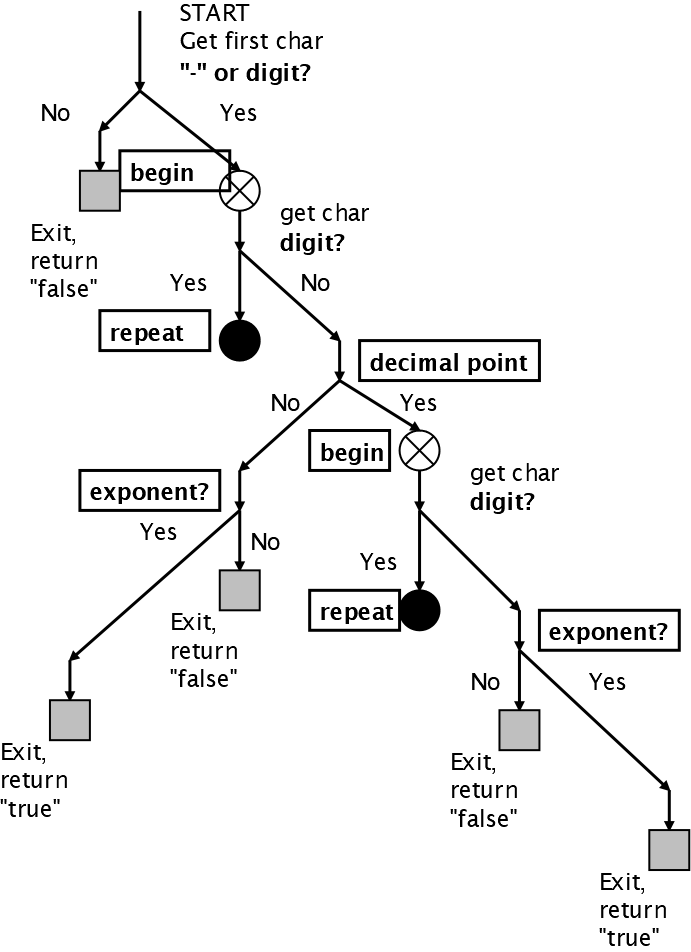
\includegraphics[width=\textwidth]{figure_11_1_diagram.png}
    \caption{Fig. 11-1 \textit{Logic tree for <floating point \#>}}
    \label{fig:11_01}
\end{figure}

and too complex either for easy comprehension or for easy maintainance\sepfootnote{11_02}.

It has been known for many years that a better way to apply general rules — \textit{e.g.}, to detemiine whether a given string conforms to the rules for "foating point number" --- uses \textbf{finite state machines} (FSMs —we define them in \ref{chap:11_02_02} below). Here is an example, written in standard FORTH:

\begin{lstlisting}
    \ determine whether the string at Sadr is a fp#
    :skip-   ( adr -- adr' ) DUP C@ ASCII - = - ;
    :skip_dp ( adr -- adr' ) DUP C@ ASCII . = - ;
    \ NOTE: these "hacks" assume "true" = -1.
    :digit?  ( char -- f ) ASCII 9 ASCII 0 WITHIN ;
    : skip_dig ( adr2 adr1 -- adr2 adr1')
        BEGIN   DDUP > OVER C@ digit? AND
        WHILE     1+  REPEAT ;   \... cont'd below
    :dDeE?   ( char -- f) 95 AND \->uppercase
        DUP ASCII D = SWAP ASCII E = OR ;

    : skip_exponent ... ; \ this definition shown below

    :fp#?    ( $adr -- f )
        DUP 0 OVER COUNT + C! \ add terminator
        DUP C@ 1+ OVER C!     \ count = count+1
        COUNT OVER + 1- SWAP  ( -- $end $beg )
        skip- skip_dig skip_dp skip_dig
        skip_exponent
        UNDER =          \ $beg' = $end?
        SWAP C@ 0= AND ; \ char[$beg']=terminal?
\end{lstlisting}

The program works like this:

\begin{itemize}
    \item Append a unique terminal character to the string.
    \item If the first character is "-" advance the pointer 1 byte, otherwise advance 0 bytes.
    \item Skip over any digits until a non-digit is found.
    \item If that character is a decimal point skip over it.
    \item Skip any digits following the decimal point.
    \item A foating point number terminates with an exponent formed according to the appropriate rule (p. 261). \bc{skip_exponent} advances the pointer through this (sub)string, or else halts at the first character that fails to fit the rule.
    \item Does the initial pointer (\$beg') now point to the calculated end of the string (\$end)? And is the last character ( char[\$beg'] ) the unique terminal? If so, report "true", else report "false".
\end{itemize}

We deferred the definition of \bc{skip_exponent}. Using conditionals it could look like

\begin{lstlisting}
: skip_exponent ( adr -- adr' )
    DUP C@ dDeE?  IF 1+ ELSE EXIT THEN
    skip- skip+
    DUP C@ digit? IF 1+ ELSE EXIT THEN
    DUP C@ digit? IF 1+ ELSE EXIT THEN
    DUP C@ digit? IF 1+ ELSE EXIT THEN ;
\end{lstlisting}

which,as we see in Fig. 11-2 below, has nearly as convoluted a logic tree as Fig. 11-1 on page 263 above.

\subsubsection{Finite state machines}\label{chap:11_02_02}

Just as we needed a FSM to achieve a graceful definition of fp\#?, we might try to define skip\_exponent as a state machine also. This means it is time to define what we mean by finite state machines. (We restrict attention to deterministic FSMs.) A finite state macliine\sepfootnote{11_03}\sepfootnote{11_04} is a program (originally it was a hard-wired switching circuit\sepfootnote{11_05}) that takes a set of discrete, mutually exclusive

\begin{figure}
    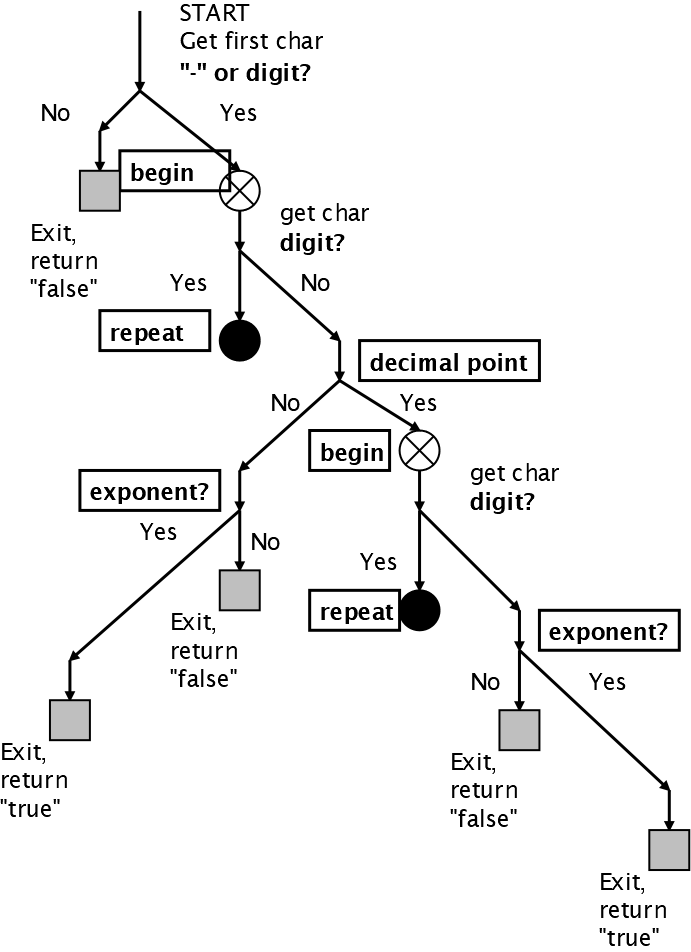
\includegraphics[width=\textwidth]{figure_11_1_diagram.png}
    \caption{Fig. 11-2 \textit{Logic tree for <exponent>}}
    \label{fig:11_02}
\end{figure}

inputs and also maintains a state variable that tracks the history of the machine's inputs. According to which state the machine is in, a given input will produce different results. The FSM program is most easily expressed in tabular form, as in Table 11-1, which we interpret as follows:

\begin{itemize}
    \item each major column heading is an input.
    \item the inputs must be mutually exclusive and exhaustive; to exhaust all possibilities we include "other".
    \item each row represents the current state of the machine.
    \item each cell contains an action, followed by a state-transition.
\end{itemize}

Table 11-1 Example of finite state machine arrow ( -> ) means 'next state'

Input:  other       dDeE        +/-         digit
State         ->          ->          ->          ->
0       Next  5     1+    1     Error 5     Next  5
1       Next  5     Next  5     1+ 2  1+    3
2       Next  5     Next  5     Next  5     1+    3
3       Next  5     Next  5     Next  5     1+    4
4       Next  5     Next  5     Next  5     1+    5

The tabular representation of a FSM is much clearer than the logic diagram, Fig. 11-2. Since the inputs must be mutually exclusive\sepfootnote{11_06} and exhaustive\sepfootnote{11_07}, there are \textit{never} conditions that cannot be fulfilled —that is, leading to "dead" code— as frequently happens with logic trees (owing to human frailty). This means the chance of introducing bugs is reduced by FSMs in tabular form.

FORTRAN, BASIC or Assembler can implement FSMs with computed GOTOs. In BASIC, \textit{e.g.},

\begin{verbatim}
    DEF SUB FSM (c$. adress)
    k% =0         ' convert input to column #
    C$=UCASE (c$)
    IF C$="D" OR C$="E" THEN k%=1
    IF C$="+" OR C$="-" THEN k%=2
    IF ASC(C$) > = 48 AND ASC(C$) < =57 THEN k%=3
    ' cont'd
\end{verbatim}

\begin{verbatim}
            ' begin FSM proper
    ON state% *3 + k% GOTO
       (0,1,2,3,4,5,6,7,8,9,10,11,12,13,14,15,16,17,18,19)
    0: state%=5
    1: adress% = adress% +1 : state% = 1
    2: CALL Error: state% = 5                          'row 0
    3: state%=5
    4: state%=5
    5: state%=5
    6: adress% = adress% +1 : state% = 2                'row 1
    7: adress% = adress% +1 : state% = 3
       ...... etc. ......
    16:state%=5
    ...... etc.......                                   'row4
    19:adress% = adress% +1 : state% = 5
    END SUB
\end{verbatim}

The advantage of FSM construction using computed GOTOs is simplicity; its disadvantage is the linear format of the program that hides the structure represented by the state table, 11-1. CASE statements —as in C, Pascal or QuickBASIC— are no clearer. We can use a state table for documentation, but the subroutine takes more-or-less the above form.

\subsubsection{FSMs In FORTH}
In the preceding FORTH example we synthesized the FSM from \bc{BEGIN...WHILE...REPEAT} loops. FORTH's lack of line-labels and GOTOs (jumps) imposed this method, producing code as untransparent as the BASIC version. The Eaker CASE statement can streamline the program,

\begin{lstlisting}
CASE: ADVANCE? NEXT 1+ ;CASE
: 1digit DUP C@ digit? ABS ADVANCE? ;
: skip_exponent (adr -- adr')
    DUP C@ dDeE? IF 1+ ELSE EXIT THEN
    skip- skip+
    1digit 1digit 1digit ;
\end{lstlisting}

(three of four \bc{IF...ELSE...THEN}s have been factored out and disguised as \bc{CASE:}...\bc{;CASE}), but this does not much improve clarity. We still need the state transition table to understand the program.

Various authors have tried to improve FSMs in FORTH using what amount to line-labels and GOTOs\sepfootnote{11_08}\sepfootnote{11_09}\sepfootnote{11_10}. The resulting code is less elegant than the BASIC version shown above.

Whenever we reach a dead end, it is helpful to return to the starting point, restate the problem and re-examine our basic assumptions One fact our preceding false starts make abundantly clear is that nowhere have we used the power of FORTH. Rather, our attempts merely imitated traditional languages in FORTH.

But FORTH is an endlessly protean language that lends itself to any programming style. Ideally FORTH relies on names so cunningly chosen that programs become self-documenting-- readable at a glance.

Since state tables clearly document FSMs, it eventually occurred to me to let FORTH compile the state table --representing an FSM-- directly to that FSM!

\TallC{Compilation} implies a \textbf{compiling word}; after some experimentation\sepfootnote{11_11} I settled on the following usage\sepfootnote{11_12}

4 WIDE FSM: (exporters)

Input: | other | dDeE | +/- I did! i
state: ———————————————————————
(0) NEXT >5 1+ >1 Error >5 NEXT >5
(1) NEXT >5 NEXT >5 1+ >2 1+ >3
(2) NEXT >5 NEXT >5 NEXT >5 1+ >3
(3) NEXT >5 NEXT >5 NEXT >5 1+ >4
(4) NEXT >5 NEXT >5 NEXT >5 1+ >5 ;

\begin{figure}
    \caption{Fig. 11-3 \textit{Form of a FORTH finite state machine}}
\end{figure}

The new defining word FSM: has a colon “ : " in its name
remind us of its function. Its children clearly must “know”
many columns they have. The word WIDE reminds us the new
created FSMs incorporate their own widths.

The column labels and table headers are merely comments fo
lowing “ \ ”; the state labels “ (0) ", “ (1 ) ", etc. arealso co
ments, delineated with parentheses. Their only purpose "
readability.

The actions \_ NEXT, Error, 1 + -in Fig. 11-3 are obvious: they;
are simply previously-defined words. But what about the state:
transitions “ > 1 ", “ > 2 ”, ? The easiest, most mnemonic and.1

natural way to handle state transitions defines them as CONSTANTs

 

O CONSTANT >0

1 CONSTANT >1

2 CONSTANT >2
etc.

which are also actions to be compiled into the FSM. This follows the:
general FORTH principle that words should execute themselves\sepfootnote{11_13}.

\TallC{In} Chapter S§2§§6 we used components of the compiler, par‘

ticularly the IMMEDIATE word ] (“switch to compile mode”),
to create self-acting jump tables. We apply the same method here:
The defining word FSM: will CREATE a new dictionary entry,
build in its width (number of columns) using “ , ”, and then
compile in the actions and state transitions as cfa’s of the ap-
propriate words.

The runtime code installed by \bc{DOES>} provides a mechanism for finding the addresses of action and state transition corresponding to the appropriate input and current state (that is, in the cell of interest). Then the runtime code updates the \textbf{state}.

11) slow nesting of FSMs (Le., compiling one into another), we
incorporate the state variable for each child FSM within its data
structure. This technique, using one extra memory cell per FSM,
protects the state from accidental interactions, since if state has
no name it cannot be invoked inadvertamly.

The FORTH code that does all this is
\begin{verbatim}
:WIDE O;
:FSM: widthon) CREATE ,,]
DOES> coI\#--)

UNDER D@    ( -- adr col\# width state)
* + 1+ 4'   ( -- adr offset )
OVER+       ( -- adr adr' )
DUP@ SWAP2+ ( -- adr [adr'] adr'+2 )
@EXECUTE    ( -- adr [adr'] state')

ROT I EXECUTE ;

O CONSTANT >0

1 CONSTANT >1

2 CONSTANT >2
.. etc.

\end{verbatim}

We are now in a position to use the code for (exponent)
(defined in Fig. 11-3 on page 269 above) to define the key

word skip\_exponent appearing in fp\#?. The result 1s

\begin{verbatim}

: skip exponent ( adr -- adr' )

' (exponent) OI \initialize state

BEGIN DUP C@ DUP (- - adr char)
dDeE? ABS OVER \input -> coI#
+/-? 2 AND + SWAP
digit? 3 AND + (--adrcol#)

' (exponent) @ \get state

5 < \ not done?

WHILE (exponent) REPEAT ;
\end{verbatim}
554 Automatic converslon tables
Our preceding example used logic to compute (not decide!) the
conversion of input condition to a column number, via

( -- char) dDeE? ABS OVER

+/-? amp + SWAP
digit? amp + ( -- col\#)


When the input condition is a character, it is usually both faster
and clearer to translate to a column number using a lookup table
rather than tests and logic. That is, we can trade increased
memory usage for speed. If a program needs many different
pattern recognizers, it is worth generating their lookup tables via
a defining word rather than crafting each by hand.
\begin{verbatim}
:TABLE: (- - #bytes)
CREATE HERE (- - #bytes tab[0] )
OVER ALLOT \ allot #bytes in dictionary
SWAP 0 FILL \ initialize to all 0's
DOES > + C@ ; ( n tab[0] - - [tab[n]])

: install (col# adr cham char.1 --) \ fast fill
SWAP 1 + SWAP
DO DDUP I+ Cl LOOP DDROP ;
\end{verbatim}
Here is how we define a new lookup table:
\begin{verbatim}
128 TABLE: [exp] \ define 128-byte table
\ modify certain chars
\ Note: all unmodified chars return col# 0

1 ASCII d ' [exp] + C! \col# 1
1 ASCII D '[exp] + Cl
1ASCII 9 '[exp] + Cl
1 ASCII E ' [exp] + Cl

2ASCII + '[exp] + Cl \col#2
2ASC|| - '[exp] + Cl

3 '[exp] ASC|l9 ASCIIO install \col#3
\end{verbatim}
With the lookup table [exp], skip\_exponent becomes faster
and more graceful,

\begin{verbatim}
: skip_exponent (adr - - adr')
' (exponent) OI \ state =0
BEGIN DUP C@ (- - adr char)
[exp] (- - adr col#)
' (exponent) @ (- - adr col# state)
5 < \ not done?
WHILE (exponent) REPEAT ;
\end{verbatim}

at a cost of 128 bytes of dictionary space. If dictionary space becomes tight, it would be perfeme simple to export the lookup

tables to their own segment. in the same way we did with generic arrays in Chapter 5.

53 Computer algebra

One of the most revolutionary recent developments in scientific
programming is the ability to do algebra on the computer.
like REDUCE. SCHOONSCIP, MACSYMA.
DERIVE and MATHEMATICA can automate tedious algebraic
manipulations that might take hours or years by hand, in the
process reducing the likelihood of error". The study of symbolic
manipulation has led to rich new areas of pure mathematics .
Here we illustrate our new tool (for compiling finite state
automata) with a rule-based recursive program to solve a problem that does not need much formal mathematical background. The resulting program executes far more rapidly on a PC than

REDUCE. e.g.. on a large mainframe.

551 Stating the problem
irac y-matrices are 0“ traceless, complex matrices defined
by a set of (anti)commutation relations 6. These are

WYV+YVVI=2vwv f.V=0.---.3 (1)
where 77‘" is a matrix-valued tensor,
p\v0 1 2 a
O I 0 O 0
”“51 O—l o o (2)
2 0 O-l O
3 O 0 O-I

274

Chapter 11 - Symbolic Proorammhg Sclendfc FORTH

The trace of a matrix is defined to be the sum of its diagonal
elements,

not ) 9 £14“ . (3)
Clearly, traces obey the distributive law

T*(A + B) E Tr(A ) + Tr(3 ) (43)
as well as a kind of commutative law,

min) a mu ). (41:)

From Eq. 1, 2, and 4a,b we find

Tr(AB) 2% [Tr(AB) +Tr(BA )] = Tip” +34)

(5)

NIH

 

=12A- 'lBTr( )=- 4A B

N"

where the ordinary vectors A " andB form the (Lorentz-in-
variant) “dot product”

A-BEAoBo—AlBl—Asz—A383 (6)

The trace of 4 gamma matrices can be obtained, analogous to
Eq. 5, by repeated application of the algebraic laws 1-4:

Tr(AB¢D) = M-BTr(¢D) — TrwA 0‘11)
Eu-BTr(¢D)-Tr(A (103) (7) '
E 4(A-Bc-D —A-CB-D +A-DB-c)

\

We include Eq. 7 for testing purposes. The factors of 4 in Eq. 5:
and 7 do nothing useful, so we might as well suppress them in the,
interest of a simpler program. -


“2 Thou.
We apply f1 rules analogous to those used in parsing a

language . The rules for traces are:
\ Gemma Matrix Algebra Rules:
\ a -> string of booth < =3
\ / - > delineator for factors
\ <factor> - > a]
\ product/ - > e/b/c/d/
\ Tr( alblprodl) - > a.b (tr( prod/) ) - tr( a/prod/b'I)
\ b' - > mark b as permuted
\ Tr( al) - > 0 (a single factor is traeeiess)

Repeated (adjacent) factors can be combined to produce a mul-
tiplicative constant:

BREE-B; (3)

recognizing such factors can shorten the final expressions sig-
nificantly, hence the rule

\ Tr( ale/prodl) - > a.a (Tr( prod/) ).

In the same category, when two vectors are orthogonal,
A -B = 0, another simplification occurs,

\ PERP A8 -> A.B=O.
\ Tr(A/B/prodl) -> -Tr(A/prod/B'/)

The ability to recognize orthogonal vectors lets us ggorrectly)
include the trace of a product times the special matrix

0010
-01 0001
Y5"yyy2y3- 1000 (9)
0100

that anticommutes with all four of the W :

ysy‘ ”“520, [I =0,...,3.

The fully antisymmetric tensor EM 2 - cw , etc., lets us write
ySAB¢EiemdA”B’C‘/‘, i=F1‘ . (10)
A complete gamma matrix package includes rules for traces contain-

ing
\ Trng( a/b/c/d/xl) - > i Tr( " /d/x/)

-> [a.b,c,d] (antisymmetric product)
\Note: "a.=".b=".c=0

 

Since y-matrices often appear in expressions like (A + m Al ) it I
will also be convenient to include the additional rules

\  *A/ -> [N + ms]
\ Tr(*A/X/) -> m[A](Tr(x/))+Tr(x/A/)

§§3 The program

We program from the bottom up, testing, adding and modifying )
as we go. Begin with the user interface; we would like to say ‘

Tf( NB/C/DI)

to obtain the output:

= A.BC.D-A.CB.D +A.DB.C ok

MM”!

own-BMW 277

Evidently our program will input a string terminated by a right
parenthesis “)”, lie, the right parsnthesis tells it to stop inputting
This can be done with the wordI

:gets ASCII) TEXT PAst 51;

Since the rules are inherently recursive, we push the input string onto a stack before operations commence. What stack? Clearly we need a stack that can hold strings of “arbitrary” length. The strings cannot be too long because the number of terms of output, hence the operating time, grows with the number of factors N, in fact. like (gr: )1 .

The pseudocode for the last word of the definition is clearly
something like

:TR( )get$ \ get a $ -terminated with ")'
setup \ push $ on $stack
parse :

\begin{figure}
    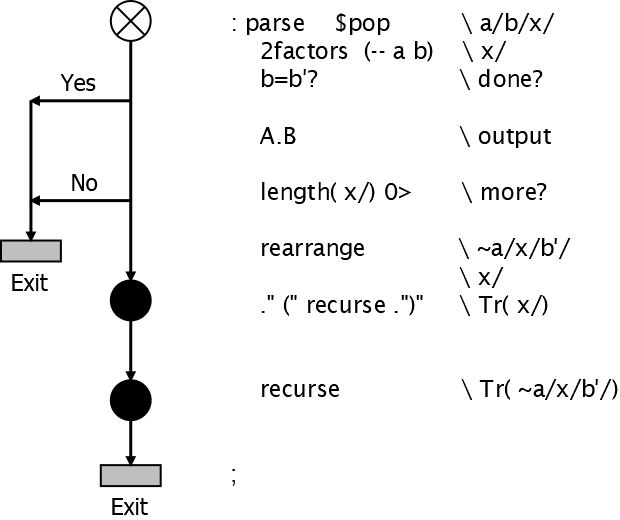
\includegraphics[width=\textwidth]{figure_11_4_diagram.png}
    \caption{Fig. 11-4 \textit{Pseudocode/flow diagram for "parse"}}
    \label{fig:11_04}
\end{figure}

Next we define the underlying data structures. Recursion
demands a stack to hold strings in various stages of decomposi-
tion and permutation. Since the number of terms grows very
rapidly with the number of factors, it will turn out that taking the
trace of as many as 20 distinct factors is a matter of some weeks
on —say— a 25 Mhz 80386 PC; that is, 14 or 16 factors are the
largest practicable number. So if we make provision for expres-
sions 20 factors long, that should be large enough for practical

purposes”.

\begin{lstlisting}
TASK GAMMA
\ FINITE STATE MACHINE
: WIDE 0 ;
: FSM: ( width 0 -- ) CREATE , , ]
    DOES> ( col# -- )
        UNDER D@        ( -- adr col# width state )
        * + 1+ 4*       ( -- adr offset )
        OVER +          ( -- adr adr1 )
        DUP@ SWAP 2+    ( -- adr [adr'] adr1+2 )
        EXECUTE@        ( -- adr [adr'] state' )
        ROT! EXECUTE    ;
0 CONSTANT >0 3 CONSTANT >3
1 CONSTANT >1 4 CONSTANT >4
2 CONSTANT >2 5 CONSTANT >5
\ END FINITE STATE MACHINE

\ Automatic conversion tables
: TAB:  ( #bytes -- )
    CREATE  HERE OVER ALLOT
            SWAP 0 FILL     \ init table
    DOES>   + C@ ;

: install   ( col# adr char.n char.1 -- )    \ fast fill
    SWAP 1+ SWAP
    DO DDUP I + C! LOOP DDROP ;
\ end automatic conversion tables

\ STRING HANDLING
HEX
\ Note: ?((( ...... ))) conditionally compiles "......"
FIND $! 0=
  ?((( : $! ( sadr dadr -- ) OVER C@ 1+  CMOVE ; )))
FIND $+ 0=
  ?((( : $+ ( adr$1 adr$2 -- pad )
    DUPC@   ( -- $adr a )
    >R 1+ OVER C@ PAD + 1+
    R@ <CMOVE PAD $!
    R> PAD C@ + 0 MAX FF MIN    PAD C! ; )))
DECIMAL
: 1+C!  ( adr -- ) DUPC@ '+ SWAP C! ;
: -BL  ( $adr -- )   \ delete all blanks from $
    DUP >R 0 PAD C! COUNT OVER + SWAP
    DO I C@ DUP@ 32 <>
        IF  PAD COUNT = C! PAD 1+C!
        ELSE DROP THEN
    LOOP    PAD R> $! ;
\ END STRING HANDLING

\ PARSE WORDS
\ Note: The factor *A/ in the input string
\ means (A/ + M sub A)
0 VAR star
: star! 123 IS star DROP ;  \ set 7th bit if 1st char=*

0 VAR #/                    \ counts # of factors
: +#/       AT #/ 1+!       DROP ; \ inc #/

: err CR -1 ABORT" Name-> letter (letter | numeral )*" ;
: +PAD ( char -- ) star OR       \ set bit 7
    PAD COUNT + C! PAD C@ '+ PAD C! 0 IS star ;
    
5 WIDE FSM: (factor)    (char col# -- )
\ input | other | letter | digit |   /   |   *   |
\ state -----------------------------------
(0)     err #0  +PAD >2  err  >0  +#/ >5  star! >1
(1)     err #0  +PAD >2  err  >1  +#/ >5  err   >1
(2)     err #0  +PAD >3  +PAD >3  +#/ >5  err   >2
(3)     err #0  +PAD >4  +PAD >4  +#/ >5  err   >3
(4)     err #0  DROP >4  DROP >4  +#/ >5  err   >4
    ;       \ terminate definition

128 TAB:    [factor]        \ convert char to col#
1 '[factor]     ASCII Z ASCII A install
1 '[factor]     ASCII z ASCII a install
2 '[factor]     ASCII 0 ASCII 9 install
3 '[factor]     ASCII / + C!
4 '[factor]     ASCII * + C!

: <factor>  (adr -- adr')
    PAD 0!  '(factor) 0! 0 IS star  \ initialize
    BEGIN DUPC@ DUP     [factor] (factor) 1+
        '(factor) @ 5 =
    UNTIL ;

CREATE factor{ 20 4* ALLOT OKLW     \ up to 20 factors
: } ( adr n - adr + 4*n) 4* + ; \ compute address

0 VAR N 0 VAR N1
CREATE  BUF$ 20 ALLOT OKLW      \ data structures

: unstar 127 AND ;  \ token[*A] = token[A] 128 OR
: $= ( $adr1 $adr2 -- f)
    -1 -ROT COUNT
    ROT COUNT ( -- $adr2+1 n2 $adr1+1 n1 )
    ROT DDUP =
    IF DROP
        0 DO  DUPC@ unstar  >R 1+
            OVER C@ unstar R>  <>
            IF ROT NOT -ROT LEAVE THEN
            SWAP 1+
        LOOP DDROP
    ELSE DDROP DDROP NOT THEN ;
: check.table ( -- )    \ prevent duplicate tokens
    -1 IS N1 LEAVE THEN
    LOOP ;

: +buf$ N N1 -1 = AND N1 -1 > N1 AND +
                                    \ token N or N1
    PAD 1+ C@ 128 AND OR            \ if star, set bit 7
    BUF$ DUPC@ + 1+ C! BUG$ 1+C! ;
                                    \ append token

: tokeniz ( $adr -- )                \ decompose into factors
    factor{ 80 0 FILL               \ initialize table
    COUNT OVER + ( -- $adr+1 $adr' ) \ addresses
    >R                  \ $adr' = $adr+LEN($) + 1
    0 BUF$ C!           \ init. buffer
    0 IS N              \ init. N
    BEGIN <factor>      \ begin loop; get factor
        check.table     \ prevent multiple entries
        +buf$           \ add factor to tokenized $
        N1 -1 =         \ not in table?
        IF PAD factor{ N } $!   \ put in table
            AT N 1+!    \ inc. N
        THEN
    DUP R@ = UNTIL      \ end loop
    DROP RDROP ;        \ clean up
\ END PARSE WORDS

\ $stack
CREATE $stack 20 20 * 2+ ALLOT OKLW     \ 2 for ptr
: $push ( $adr -- )
    DUPC@ 19 > ABORT" STRING TOO LONG!"
    $stack DUP@ DUP 19 > ABORT" $stack too deep!"
    20 * 2+ + $!    $stack 1+! ;
: $pop  ( $adr -- ) $stack DUP@ 1- 0 MAX
    DDUP SWAP !
    20 * 2+ + SWAP $!
\ end $stack

CREATE X$ 80 ALLOT OKLW \ buffer for input $, tail$
: get$ ASCII ) TEXT     \ input a $ terminated by )
    PAD -BL             \ delete blanks
    PAD X$ $! ;

: 1factor ( -- a )      \ get 1 factor, tail -> x$
    BUF$ 1+ C@          ( -- a )
    BUF$ COUNT 1- >R
    1+ X$ 1+ R@ <CMOVE  \ tail -> x$
    R> X$ C! ;          \ adjust count
: 2factors ( -- a b )   \ get 1st 2 factors
    1factor X$ BUF$ $! 1factor ;

0 VAR sign              \ emit correct sign
2 TAB: [sign]           \ make table
ASCII + '[sign]    C!   \ fill table
ASCII - '[sign] 1+ C!
: .sign ( a -- ) 64 AND 0> [sign] sign AND EMIT ;

\ Note: we mark prime (') by 64 OR (set bit 6 in token)
\   since 1st factor is never ', we set bit 6 for leading "-" sign
: prime!    64 OR  ;
: unprime   63 AND ;
: A.B   ( a b -- )      \ emit "dot product"
    unprime             \ b' -> b
    OVER .sign          \ emit sign
    SWAP unprime        \ drop leading "-"
    DDUP MAX -ROT MIN   \ sort factors
    factor{ SWAP } $.
    ASCII . EMIT factor{ SWAP } $.  -1 IS sign ;

: clean ( $adr -- )     \ unprime all factors
    COUNT OVER + SWAP
    DO I C@ unprime I C! LOOP ;


: rearrange      ( a b -- )
    1 BUF$  \ init buf$
    BUF$ X$ $+ PAD BUF$ $!       \ buf$-> _/x/
    prime!          ( -- a b' )
    BUF$ COUNT + C! BUF$ 1+C!    \ buf$-> _/x/b'/
    64 XOR       ( -- a xor 64 ) \ toggle sign of a
    BUF$ 1+ C! ; ( -- )          \ buf$-> ~a/x/b'/

: setup     X$ tokenize         \ form token$
            $stack 0!           \ init $stack
            0 IS sign           \ init sign flags
            BUF$ $push ;        \ input token$ on $ stack

\                               debugging code
: $$.   ( $adr -- ) COUNT OVER + SWAP   \ translate token$
    DUPC@ .sign factor{ OVER C@ unprime } $. ."/"
    1+ DO   factor{ I C@ unprime } $.
            I C@ 64 AND 0>              \ primed?
            IF ." '" THEN   ."/"
    LOOP ;
: dump$stack? DEBUG NOT IF EXIT THEN
    $stack 2+       ( -- $adr[0] )
    $stack @ DUP 0= \ $stack empty?
    IF DDROP CR ." $stack empty" EXIT THEN
    0 DO I 20 * OVER + CR $$. LOOP DROP ;
0 VAR DEBUG
: DEBUG-ON  -1 IS DEBUG ;
: DEBUG-OFF  0 IS DEBUG ;
\               end bebugging code

: (.    ."("  0 IS sign ;
: ).    .")" -1 IS sign ;
: parse dump$stack?
    BUF$    $pop    2factors ( -- a b )
    DUP     64 AND 0>        \ b = b'?
    IF      DDROP EXIT THEN
    DDUP A.B    ( -- a b )   \ output
    X$ C@ 0>                 \ more?
    IF  rearrange   \ buf$=    ~a/x/b'/
        BUF$ $push           \ ~a/x/b'/
        X$ clean X$ $push    \    x/
        (. RECURSE ).
           RECURSE
    ELSE    DDROP   THEN ;

: TR(   get$                 \ input $
        setup
        ." =" CR             \ for beauty
        parse ;
\end{lstlisting}

Since the tokens are 1-byte integers smaller than 32, their 5th, 6th, and 7th bits can serve as flags to indicate their properties. For example, we need to indicate whether a factor was "starred", \ie. whether it represents $(\tr{A} + m_{A}I)$ or $\tr{A}$ , according to the rule
 

.' (' recurse .')" \ Tr(x/)

 

recurse \ Tr( "' a/x/b'l)

 

Exit

 

 

Fig. 11-4 Pseudocode/fow diagram for ‘parse'

How deep an the Sstack get? The algorithm expressed by the rule
\ Tr( a/b/prodl) - > a.b ( Tr( prodl) ) - Tr( a/prod/b'l)

suggests that for an expression of length n=2k, the maximum
depth will be k + 1. Thus we should plan for a stack depth of at
least 11, perhaps 12 for safety. Assuming factor-names up to three
characters long, and strings of up to 20 names, we need =60
characters per string. My first impulse was to create a dynamic
\bc{$stack} that could accomodate strings of variable length, meaning
that some 330 bytes of storage would be needed, at the cost of
some complexity in keeping track of the addresses. This is a big
improvement on 720 bytes needed for a 60-wide fixed-width
stack, of course. However, the convenience of a fixed-width
Sstack led me ultimately to set up a table (array) of 20 names,
whose indices would act as tokens; that is, the strings that actually
go on the Sstack would be tokenized. The memory cost of the
table together with a 12-deep, fixed-width Sstack is thus only
80 + 242 = 322 bytes.

\begin{verbatim}
(0) arr >0 wan >2 err >0 +0! >5 _!>1
(1) on >0 4PM >2 an >1 +OI>5 en >1
(2) on >0 4?“) >3 +PAD >3 +0! >5tr >2
(3) 01" >0 OPPD >4+PND >4 +O/ >5” >3
(4) on >0 W umf 40/ >Sarr>4
\end{verbatim}

Since the tokens are 1-byte integers smaller than 32, their 5th, 6th
and 7th bits can serve as fags to indicate their properties. For
example, we need to indicate whether a factor was “starred”, Le.

whether it represents (A + mAl) or A , according to the rule
\ A / -> (N+m[A)).

Again, we need to be able to indicate a “prime", showing that a
factor has been permuted following the rule

\ TI’(8/b/Pf°d/) -> lbiNPVOUO) ~"(9/P'06/b'0

Thus we set bit 7 (128 OR) to indicate “star", and bit 6 (64 OR)
to indicate “prime".

We still need to indicate the leading sign. My first impulse was to
use bit 5, but I realized the first factor is never permuted, hence
its 6th bit is available to signify the sign. It is toggled by the phrase
84 XOR. (In the Sstack pictures appearing in the Figures we
indicate toggling by a leading “ "‘ ”.)

Programming these aspects is fairly trivial so we need not dwell
on it. The entire program appears on pages 279 and 280 above.

Now we test the program:

rm NB/C/D/E/f) =
A.B(C.D(E.F)—C.E(D.F) + C.F(D.E))
—A.C(D.E(B.F)—D.F(B.E) + B.D(E.F))
+A.D(E.F(B.C)—B.E(C.F) +C.E(B.F))
-A.E(B.F(C.D)-C.F(B.D) + D.F(B.C))
+A.F(B.C(D.E)—B.D(C.E) + B.E(C.D)) ok

Clearly the concept works. Our next task is to incorporate

branches to take care of “starred”, as well as identical and/or
orthogonal adjacent factors. The possible responses to the dif-
ferent cases are presented in decision-table form in Table 11-2:

To avoid excessively convoluted logic we eschew nested branch-
ing constructs. A finite state machine would be ideal for clarity;
however, as Table 11-2 makes clear, the logic is not really that of
a FSM, besides which, the FSM compiler described above would

OJlfanVNoHoim—Altigfamorvad.

 

 

1put: a/b/x/ 'a/b/x/ al‘h/x/ a/a/x/ a/b/xl. i
ab=0

asulting "' a/x/b'l a/b/x/ a/b/XI

stack: XI b/XI a/x/ x/ "' a/x/b’l

iction(s)T: a.b m[a] m[b] a.a RECURSE

 

(necunse) (necunsa) (necunse) (ascunse)

RECURSE RECURSE RECURSE

 

Note: characters shown in light typeface are EMthed.

 

have to be modified to keep its state variable on the stack, since
otherwise it could not support recursion. The resulting pseudo-
code program is shown in Fig. 11-5. Implementing the code is now
straightforward, so we omit the details, such as how to define
PERP to appropriately mark the symbols. The simplest method
is a linked list or table of some sort, that is filled by PEHP and
consulted by the test word perps?.

ow might we implement a leading factor of y5? While there
is no difficulty in taking traces of the form

Tr( 1'54 18 af ...) a iTr(e,..aA"B ’c‘y‘n ...), (11)

expressions with y5 between "starred" factors are more difficult.
However, the permutation properties of traces let us write, e.g.,

Tr((A +mA)(B+mB)y5¢(D+mD)E...)
(12)

ETI(YS¢(D+MD)E---(A +mi)(B+ms)).

\begin{figure}
    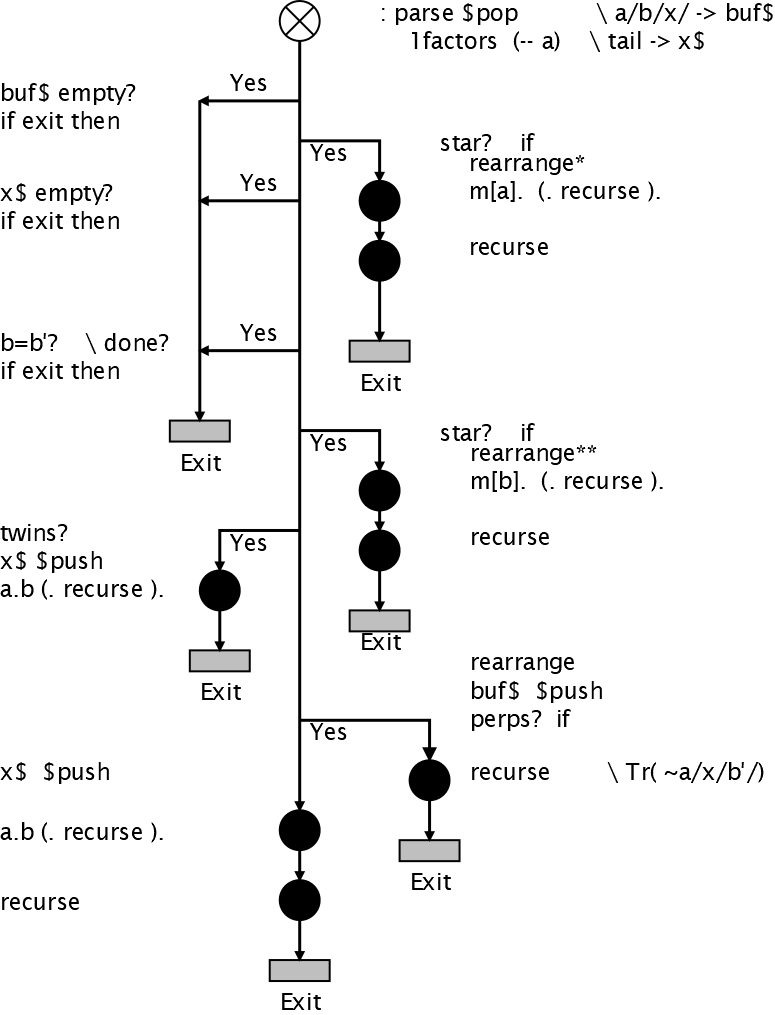
\includegraphics[width=\textwidth]{figure_11_5_diagram.png}
    \caption{Fig. 11-5 \textit{Pseudocode/flow diagram for extended "parse"}}
    \label{fig:11_05}
\end{figure}

so the key issue becomes decomposing leading starred factors, saving the pieces on the \$stack until at least three distinct unstarred factors are adjacent on the left. Replace these by a special 

The only other significant task is to extend the output routine to ‘

a) recognize the special “ " ” token; and
b) replace dot products like “ " .d ” by [a,b,c,d].

A final remark: one or another form of vectoring can simplify
parse (relative to Fig. 11-5) by hiding the recursion within words
that execute the branches. We have avoided this method here

because it conceals the algorithm, a distinct pedagogical disad-
vantage.

FORmula TRANslator

That prehistoric language FORTRAN -despite its manifold
deficiencies relative to FORTH — contains a useful and widely
imitated invention that helps maintain its popularity despite come
petition from more modern languages: This is the FORmula
TRANslator from which the name FORTRAN derives.

FORTH’s lack of FORmula TRANslator is keenly felt. Years of
scientific FORTH programming have not entirely eliminated my
habit of first writing a pseudo-FORI'RAN version of a new algo-
rithm before reexpressing it in FORTH. Sometimes I will even
write a test program in QuickBASIC‘D before re- coding it in
FORTH for speed and power, just to avoid worry about getting
the arithmetic expressions correct.

l
imam

awn-BMW 285

III mum

A FORmula TRANslator provides a nice illustration of rule-

d programming. To maintain portability, we employ the
standard FORTH kernel, omitting special HS/FORTH words as
well as CODE words.

In principle we could provide a true compiler that translates
formulae to machine code (or anng, to assembler). But unless
we use p-code or some such artifice we would lose all hope of
portability. Thus, we take instead the simpler course of translating
FORTRAN formulae to FORTH according to the rules

\begin{verbatim}
\ NUMBERS:

\ <int> -> -| 0} {digit digit"8}

\ <exp't> -> dDeEI{& | 0} {digit digit"2}| 0}
\ <fp#> -> -|O} dig | Q} . dig" <exp't>
\ FORMULAS:

\ <assignment> -> <subject> = <expression>

\ <id> -> letter {ietter|digit}"6

\ <subjec1> -> <id>{<id|ist>10}

\ <idiist> ->(<id> {,<id> ")

\ <arglist> ->(<expr'n> {,<expr’n> }")
\ <function> -> <id> <arglist>

\ <expression> -> <terrn> | < term> at <expr'n>
\ <term> _> <factor> | <tactor> 96 <term>
\ <factor> -> <id>| <tp#>| (<expr'n>) |
\end{verbatim}

-> <factor> “ <iactor>

Clearly, the FORTH FORmula TRANslator could become the
kernel of a more complete FORTRAN- >FORTH filter by ad-
ding to the above rules for formulae the following rules for loops
and conditionals:

\begin{verbatim}
\ DOLOOPS:

\ <label> -> <integer>
\ <lim> -> <integer>|<id>}
\ <step> -> ,<lim>|O}

\ <do> -> DO<label><id>=<iim>,<lim><step>

\ BRANCHING STRUCTURES:
\ < logical expr > - > <factor > .op. < factor >
\ <il0> -> IF(<Ioglcalexpr>)<assignment>
<if1 > -> IF(< logical expr>)THEN
{< statement > } "
END IF

<if2> -> lF(<Iogical expr>)THEN
{ < statement > } "
ELSE
{ < statement > } "
END IF


- > IF ( < logical expr > )THEN
{ < statement >} "
ELSEIF( < logical expr >)
{ < statement > } A
END IF

\end{verbatim}

§§2 Details of the Problem
The general principles of compiler writing are of course well
understood and have been described extensively elsewhere. ..
Several computer science texts expound programs for formula ‘
evaluators . Once we have our translator, we can easily make it
an evaluator by compiling the FORTH as a single word, then
invoking it.

 

Let us proceed by translating a FORTRAN formula into FORTH
code by hand. For simplicity, ignore integer arithmetic and as-
sume all literals will be placed on the intelligent foating point
stack (ifstack). Similarly assume all variable names in the pro- ,
gram refer to SCALARs (see Ch. 5). A word that has become
fairly standard is 96, which interprets a following number asE
foating point, and places it on the fstack. With these conventions,
we see that we shall want to translate an expression like

A - -15.3€7'EXP(7/X) + Z/(W-SINUHETA'Pl/lmyf
into (generic) FORTH something like this:

964 REAL’B >FS
96 1M REAL'B >FS
Pl G\

THEl’A >FS G‘
GSIN G

W >FS G -

Z >FS G\

X >FS

967 REAL'B G\
GEXP

96 45.357 REAL‘B >FS
Gt

G+

A FS>

Begin with the user interface. We will define a word, F' , that
will accept a terminated string and attempt to translate it to
FORTH. That is, we might say

F- A = -15,3E7*EXP(7/X) +Z/(W-SIN(THETA'PI/180)/4)'

and obtain the output (actual output from the working program!)

96 -15.3E7 REALM F>FS 96 7 REAL‘B F>FS
X>FS G/ GEXP G* Z>FS W>FS
THETA >FS Pl >FS G‘ 96 180 REAL‘B F>FS
G/ GSIN 96 4REAL‘8 F>FS G/ GNEGATE
G-l-G/ G+ AFS> 0k

Although the second version differs somewhat from the hand
translation, the two are functionally equivalent.

We would also like to have the possibility of compiling the emitted
FORTH words, if F' appears within a colon definition, as in

: do.B F' B = 39.37/ATAN(X“W) + 7"Z/X' ;

FORTRAN expression obeys the rules of algebra in a general-
y obvious fashion. Parentheses can be used to eliminate all
ambiguity and force a definite order on the evaluation of terms

esuuvuouoiaaa-Mmm.

Chapter 11 — Symbolic Programming Scientific FORTH

and factors. However, to reduce the number of parentheses,
FORTRAN adopted a heirarchy of operators that has been fol-
lowed by all other languages that incorporate semi-algebraic
replacement statements like the above. The heirarchy is

0. FUNCTION

1. EXPONEN'TIATION ( A or u)
2. t or/

3. + or —

4. “ , ” (argument separator in lists)

The translator must both enforce these rules and resolve am-
biguities involving operators at the same heirarchical level. Thus,
e.g., does the fragment

NB‘C

mean N(B*C) or (NB)*C ? Many FORTRAN compilers follow
the latter convention, so we will maintain this tradition.

Wd issue is the function library. The FORmula
slator must recognize functions, and be able to deter-
mine whether a given function is in the standard library. In the
example above, F" recognized EXP and SIN as standard library
functions and emitted the FORTH code to invoke them. Abeauty
of FORTH is that there are several easy ways to accomplish this,
using components of the FORTH kernel.

A third issue is the ability of a true FORTRAN compiler to
perform mixed-mode arithmetic, combining INTEGER'Z, IN-
TEGER‘4, INTEGER'8, REAL‘4, REAL'S, COMPLEX'S
and COMPLEX' 16 types ad libitem. FORTRAN does this using
the information contained in the type declarations at the begin-
ning of a routine. A pure FORmula TRANslator has no such
noncontextual information available to it, hence has no way to
decide how to insert the proper FORTH words during compila-
tion. To get around this we employ the generic data and operator
conventions developed in Chapter 5 §l.

swimmer" awn-OMW 2”

"3 Pm
Let us hand-parse the example, reproduced below:

A I -15.3€7'EXP(7/X) + Z/(W-SINCI'HETA'PII 1N)/4)

Clearly, we must apply the first rule

\ <assignment> -> <subiect> n <expression>

embodied in the word < assignment > . We split at the “ = " sign,
and interpret the text to its left as a SCALAH. Since we want to
emit the phrase A FS > last, yet have parsed it first, we have to
hold it somewhere. Clearly the buffer where we store it will be a
first-in last-out type; and by induction, last-in, first-out also. But
a LIFO buffer is a stack. Hence the fundamental data structure
needed in our parsing algorithm is a string stack. So we might
imagine that after the first parsing step the string stack contains

 

two strings
£SIACK Notes
A FS > \ < subject >

-15.3E7*EXP(7/X) + Z/(W-SlN('l’HETA"P|/180)/4) \ < expressio

Next we apply the rule
\ <expr'n> -> <term> |<term> a <axpr'n>

This breaks the top expression at the + sign between “ ) " and Z.
We should think of the two terms

-15.3E7*EXP(7/X)

and

Z/(W-SINUHETNPIMBOW)

as numbers on the ifstack; hence the code to evaluate each should
be emitted before the addition operator (that is, these expres-
sions are higher on the string stack than the addition operator
0 +). We adopt a rule that the right term is pushed before the
left, so the Sstack now looks like

emvuounm-umm.

Chapter 11 - Symbolic Programming Sclemlfc FORTH

 

SSIAQK Notes

A FS > \ < subject >
Z/(W-SIN(THETA*PI/180)/4) G + \ <term >
-15.3E7*EXP(7IX) \ < term >

We now anticipate a new problem: suppose we have somehow —
no need to worry about details yet — emitted the code for the
< term > -15.3E7*EXP(7/X) on top of the Sstack. Then we
would have to parse the line Z/(W-SINCI’ HETA'Pl/1 80)/4) G + .
Assuming the program knows how to handle the first part,
Z/(W-SIN(THETA"PI/180)/4), how will it deal with the G + ?
We do not want to use the space as a delimiter (an obvious out)
because this will cause trouble with A FS > .

The difficulty came from placing 6+ on the same line as
—1 5.3E7‘EXP(7/X). What if we had placed the operator on the
line above, as in

 

SSIACK Notes

A FS > \ < subject >
G + \ operator
Z/(W-SINUHETA'PI/180)/4) \ < term >
-15.3E7*EXP(7/X) \ < term >

Eventually we see this merely exchanges one problem for another
of equal difficulty: How do we distinguish a < factor > or
< term > that contains no more operators or functions — and is
therefore ready to be emitted as code — from the operator G +,
which contains a “ +” sign? Now we need complex expression
recognition, which will lead to a slow, complicated program.

When this sort of impasse arises (and I am pretending it had

been realized early in the design process, although the dif-
ficulty did not register until somewhat later) it signals that a key
issue has been overlooked. Here, we failed to distinguish FORTH
words, FS > and G +, from FORTRAN expressions. We have, in
effect, mixed disparate data types (like trying to add scalars and
vectors). Worse, we discarded too soon information that might

have been [BCfUI at a later stage. This leads to a programming tip,
a la Brodie :

I m: Never discard information. You might need it later.

Phrased this way. the solution becomes obvious: keep the
operators on a separate stack. whose level parallels the expres-
sions. So we now envision an expression stack and an operator
stack, which we call 13/8 and 0/5 for short. On two stacks,

 

E/S Q15 Notes
A FS > \ < subject >
Z/(W-SINCI‘HETA'Pi/180)/4) G + \ < term >
—15.3E7"EXP(7/X) NOP \ < term >

Why the NOPs (“no operation”) on the 0/8? We want to keep
the stack levels the same (so we do not have to check when
POPping off code strings); we thus have to put NOP on the 0/5
to balance a string on the BS.

The IDS now contains a < term > , so we apply the rules
\begin{verbatim}
\ <function> -> <id> <arglist>
\ <term> -> <iactor> | <factor> 96 <term>

\ <factor>-> <id>| <fp#>| (<expr’n>) |<func>
\end{verbatim}

We note there is an operator at the “ 96 " priority level (the “a"
in the TOS). We split the top < term > at this point, issuing a G'.

 

EIS QLSN.QIQ§
A FS > \ < subject >
Z/(W-SINO’HEI'A'Pl/180)/4) G + \ < term >
EXPO/X) G‘ \ (term >
-1 5.367 NOP


The parsing has now reached a turning point: the top string on
the E/S can be reduced no further. The program must recognize
this and emit the corresponding line of code (sec Ch. 5):

% —15.3E7 REALM F>FS

 

leaving

E18 018 Notes
A FS > \ < subject >
Z/(W—SIN (T HETA*P|/180)/4) G + \ < term >
NULL 6*
EXP(7/X) NOP \ < function >

What is NULL and why have we pushed it onto the E/S? Simply,
it is not yet time to emit the 6" so we have to save it; however,
we have another operator, G +, to associate with Z/(W-
SlN(THETA*PI/180)/4) . Thus we have no choice but to define a
placeholder for the 13/5, analogous to NOP on the 0/5.

S now contains a function. Assuming we can recognize it as
such, we want to check that it is in the library and put the
correct operator on the 13/5. Thus we want to decompose to

 

E15 018 Notes
A FS > \ < subject >
Z/(W-SIN(THETA*P|/180)/4) G + \ < term >
NULL 6*
NULL GEXP \ < function >
(7 IX) NOP \ < arglist >

The parentheses around the <arglist> on TOS serve no pur-
pose, so drop them.

We see, once again, an operator of the priority-level 96 (the “I”
between 7 and X), so we again apply the rule

\ <term> -> <factor> | <factor> 9i. <term>

to obtain

El: 013 Item

A F8 > \ < subject >
ZlM-SlNCFHETA'Pi/iwyf G + \ < term >
NULL G“

NULL GEXP

X G] \ < id >

7 NOP \ < ip\# >

Once again we can emit a number, so we do it:

96 7 REAL'B F> FS

Wait! Why did we say REALM with —15.3E7, but REAL'B with
7 just now? Can’t we make up our minds? The answer is that we
want to respect precision over-rides via FORTRAN's E (single
precision, so we say REALM) or D (double precision — REAL'B)
exponent prefixes. However, where we are free to choose, it
makes sense to keep maximum precision.

We continue, emitting the next simple items on the Sstack:

X G/ GEXP G‘

 

leaving

E18 018 Notes
A FS > \ < subject >
Z/(W-SlNCI’HETA'PI/180)l4) G + \ < term >

Once again we find the most exposed operator to be “ / which
we split with the rule

\ <term> -> <factor> | <factor> 96 <term>

 

E/S QLSN91§§

A FS> \ <subject>
NULL G + \ < term >
(ZW~SIN(THETA*Pi/180)/4) Slop \ ( < expr > )

Chapter 11 - Symbolic Programming Scientific FORTH

Emit the T082
2 > PS
and apply the rule (first drop the parentheses)

\ <expr'n> -> <term> | <term> a <expr'n>

 

EIS Q15 Nona
A FS > \ < subject >
NULL G + \ < term >
NULL G/
—SIN(THEl'A*PI/180)/4 G +
W NOP

Why did we issue G + and keep the leading “—” sign with SIN?
Simple: any 9th grader can tell the difference between a “—”
binary operator (binop) and a “—” unary operator (unop) in an
expression. But, while not impossible, it is unnecessarily difficult
to program this distinction. The FORTH philosophy is “Keep it
simple!” Simplicity dictates that we embrace every opportunity
to avoid a decision, such as that between “—” binop and “-" unop.
The algebraic identity

X—YEX+(—Y)

lets us issue only G + , as long as we agree always to attac “—”
signs as unops to the expressions that follow them. Eventually,
of course, we shall have to deal with the distinction between
negative literals (-15.3E7, e.g.) and negation of variables. The
first we can leave alone, since the literal-handling word 96 (“treat
the following number as foating point and put it on the 87stack”)
surely knows how to handle a unary “—" sign; whereas the second
case will require us to issue a strategic GNEGATE.

A consequence of this method for handling “-” signs is that the
compiler will resolve the ambiguous expression

—X" =9 -(X") or (—X )Y

Mir-WW 295

in favor of the former alternative. if the latter is intended, it must
be specified with explicit parentheses.

After sending forth the phrase
W > PS

the leading “-" preceding SIN( ...)/4 must be dealt with. To
preserve the proper ordering on emission we will want a word
LEADING- that puts the token for GNEGATE on the 0/8 and
moves the string SiNCl'i-iETA'PI/i 00)“ to the TOS, issuing a
NOP on the BS, obtaining

 

E18 018 Ngtgs
A FS > \ < subject >
NULL G + \ < term >
NULL 6/
NULL G +
NULL GNEGATE
SIN (THETA'Pl/1 80)/4 NOP

The next exposed operator is at“ 96 " -level. We apply < term >
once more, to get:

 

EIS OLS Notes
NULL GNEGATE
4 G/
SINO‘HETA'PIHBO) NOP \ ( <expr'n> )

After handling the function as before we find the successive stacks
and FORTH code emissions

 

E/S MS Notes
A FS > \ < subject >
NULL G + \ < term >
NULL 6/
NULL G +
NULL, GNEGATE
4 GI
NULL GSIN

(THETA'PI/180) NOP

Chapter 1 t - Symbolic Programming Scientific FORTH

 

51 0/8 Joins
A FS > \ < subject >
NULL G + \ < term >
NULL 6/
NULL G +
NULL GNEGATE
4 GI
NULL GSIN
180 6/
PI 6*
THETA NOP

THETA >FS PI >FS G“ 96180 REAL*8 F>FS
G/ GSIN %4 REAL‘B F>FS G/ GNEGATE G+
G/ G+ AFS> ok

4 Coding the FORmula TRANslator

e proceed in the usual bottom-up manner. The first question

is how to define the Sstack. In the interest of brevity, I chose
not to push the actual strings on the E/S, but rather pointers to
their beginnings and ends. By using a token to represent the
operator, we can define a 6-byte wide stack which will point to
the text of interest (which itself resides in a buffer), and will hold
the token for the operator at the current level. This way only one
stack is pushed or popped and the levels never get out of
synchronization.

Again at the lowest level, we can develop the components that
recognize patterns, e.g., whether a piece of text is a foating point

number. The word that does the latter is \bc{fp\#?}, already described
in §2§§1.

A function is defined by the rule

\ <arglist> -> ( <expr'n> {, <expr'n>}")
\ <function> -> <id> <argl|st>

We may therefore identify a function by splitting at the first left
parenthesis,

\begin{lstlisting}
    : >(    ( $end $beg -- $end $beg' ) \ find first "("
        1- BEGIN 1+ DUPC@ ASCII ( = >R
              DDUP = R> OR UNTIL ;
\end{lstlisting}

and then applying appropriately defined FSMs to determine
whether the pieces are as they should be.

:<thction>($endSbeg--i)
DUP>R >( (--Send$beg')
UNDER 1- Fi> <id>

—ROT SWAP <arglist> AND ;

The FSM < argllct > must be smart enough to exclude cases such
as

SIN(A + B)/(C-D)
and
SIN(A + B)/EXP(C-D)

that is, compound expressions that might contain functions; it
must also correctly recognize, e.g.,

SIN((A + B)/EXP(C-D))

as a function.

In FORTH there is no distinction between library functions and
functions we define ourselves. In either case, the protocol defined
in Chapter 8 will work fine. Thus the code generator for < func-
tion > emits the code

USE( fn.name arg1 argz argN F(x)

What, however, do we do about translating standard FORTRAN
names such as SIN, COS and EXP to their generic FORTH
equivalents? The simplest method defines words with the names
of the FORTRAN library functions. The FORTH-83 word FIND
locates the code-field address of a name residing in a string. Thus
we could have (note: .GSIN is a CONSTANT containing a token)

.GSIN CONSTANT sm \etc.

omvmtm-umm.

298 Chapter 11 — Symbolic Programming Scientific FORTH

:LIBRARY? ($end$beg--cta | 0)
—ROT UNDER — DUP>R
PADt+ SWAP CMOVE R> PAD CI \ makes
PAD FIND (--cia n) o= NOT AND ;

now we can define function! which, assuming pointers to the
< id > and < arglist > are on the stack, rearranges the Sstack like

 

 

this:
BS QIS Notes
(argt, argz, argN) .F(X) \ an op.
NULL .iib\_name \ if library function
or, if it is a user-defined function, like this:
E18 018 Notes
(arg1, argZ, argN) .F(X) \ an op.
name NOP \ user function

The code that does all this is

\begin{lstlisting}
: function! ($end2 $beg2 $end1 $beg1 - -)
.F(X) $push \ push arglist
DDUP LIBRARY? DUP 0=
IF DROP .NOP $push \ userfn
ELSE EXECUTE \ inlib.
NULL ROT $PUSH DDROP
THEN ." USE( " ;
\end{lstlisting}

For the program itself24 we work from the last word, < aslgn-

ment > , to the first (which we do not know the name of yet).
We shall describe the program in pseudocode only, in the interest
of saving space. Clearly,

\begin{lstlisting}
: < assignment > \ input $ assumed in buffer
<subj> = <expr> \ splitat "=" (- -t)
IF subjl THEN \ put Subj and its code on $staci<
.NOP $push ; \ then put expr on Sstack
\end{lstlisting}

Certain decisions need to be made here: for example, do we want
F' to be able to parse an expression that is not an assignment (that
is, generating code which evaluates the expression and leaves the
result on the ifstack)? We allowed this with the IF...THEN.

Next we pseudocode < oxproeeion >:
: <expression> empty? IF EXIT THEN
59°F


IF trm\&exprl RECURSE
ELSE NULL ROT $push
.NOP $push <term>
THEN ;

Defined recursively in this way, < oxpreoolon > will keep
working on the TOS until it has broken it up into term 5.

We similarly define < term > recursively, so it will break up any
term 5 into all their factors. It should also recognize < arglist > 5.
Thus:

: <term> empty? IF EXIT THEN

$pop < arglist >$
IF arglist! < expression > EXIT THEN
<factor>\%<term> (--f)\ splitat\%="/'

IF fct%trml RECURSE
ELSE .NOP $push$ <factor> \ term = factor
THEN ;

And finally, we define < factor > , again recursively,
\begin{lstlisting}
: <factor> empty? IF EXIT THEN \ done
SPOP <fp# > \ fp#?
IF fp#I RECURSE EXIT THEN
leading -?
IF leading-I < expression > \ forward ref.
EXIT THEN
< id > IF idI < expression > \ forward ref.
EXIT THEN
<f>"<f> \ exponent'?
IF f"fi RECURSE RECURSE
EXIT THEN
\ oont'd

< function >
IF functionl < expression > \ forward ref.
EXIT THEN

(< expression >) \ expression inside ( )?

IF exposel < expression > \ forward ref.
ELSE ." Notafactorl' ABORT THEN ;
\end{lstlisting}

Note the forward references found in \bc{<factor>}; since \bc{<expression >} is defined later, we must use vectored execution or some similar method to permit this recursive call.

With this we conclude our discussion of rule-based programming. The complete code for the FORmula TRANslator is too lengthy to print, hence it will be found on the included diskette.